\documentclass{entcs}
\usepackage{entcsmacrosasb}
\usepackage{graphicx}
\usepackage{amsmath}
\usepackage{calc}
\usepackage{mathtools}
%\usepackage{subcaption}
\usepackage{kappa}
\usepackage{xypic}
\usepackage{subfigure}
\usepackage{stmaryrd}
\usepackage{boolean}
\sloppy
% The following is enclosed to allow easy detection of differences in
% ascii coding.
% Upper-case    A B C D E F G H I J K L M N O P Q R S T U V W X Y Z
% Lower-case    a b c d e f g h i j k l m n o p q r s t u v w x y z
% Digits        0 1 2 3 4 5 6 7 8 9
% Exclamation   !           Double quote "          Hash (number) #
% Dollar        $           Percent      %          Ampersand     &
% Acute accent  '           Left paren   (          Right paren   )
% Asterisk      *           Plus         +          Comma         ,
% Minus         -           Point        .          Solidus       /
% Colon         :           Semicolon    ;          Less than     <
% Equals        =3D           Greater than >          Question mark ?
% At            @           Left bracket [          Backslash     \
% Right bracket ]           Circumflex   ^          Underscore    _
% Grave accent  `           Left brace   {          Vertical bar  |
% Right brace   }           Tilde        ~

% A couple of exemplary definitions:

\newcommand{\map}[2]{#2}
\newcommand{\todo}[1]{{\huge\textcolor{red}{#1}}}
\newcommand{\todoo}[1]{{\large\textcolor{green}{#1}}}
\newcommand{\keep}[3]{#1{#2}{#3}}
\letboolval{\explainweakembedding}{\FALSE}
%\newcommand{\binomial}[2]{\left(\begin{array}{c}\scriptstyle #2\cr \scriptstyle #1\end{array}\right)}
\newcommand{\binomial}[2]{{{#2}\choose{#1}}}
\newcommand{\validannotations}[1][EP]{\llbracket EP \rrbracket}
\newcommand{\realisationsaux}[2][EP]{\llbracket #2 \rrbracket_{#1}}
\newcommand{\realisations}[1][\phi]{\realisationsaux{#1}}
\newcommand{\canonic}{\bigcup \realisations}
\newcommand{\card}[1]{\sharp#1}
\newcommand{\Nat}{{\mathbb N}}
\newcommand{\Real}{{\mathbb R}}
\newcommand{\eps}[1]{}
\newcommand{\freesymbol}{\dashv}
\newcommand{\freeindex}[1]{%
\def\arga{#1}%
\if\arga0
\,\freesymbol\!
\else
\freesymbolrev\,
\fi}
\newcommand{\boundsymbol}{-}
\renewcommand{\bound}[1]{\boundsymbol}
\newcommand{\boundsymbolrev}{\boundsymbol}
\newcommand{\species}[3]{#1{0}A_#3#2{1}}
\newcommand{\rhodot}[3]{[\species{#1}{#2}{#3}]_e}
\newcommand{\conc}[3]{[\species{#1}{#2}{#3}]}
\newcommand{\concshort}[1]{[#1]}
\newcommand{\eg}{e.g.~}
\newcommand{\ie}{i.e.~}
\newcommand{\graphsymb}{G}
\newcommand{\iso}{\approx}
\newcommand{\rembedding}[1][]{\xymatrix@C=0.35cm{{}\ar@{^{(}->}[r]^{#1}&{}}}
\newcommand{\lembedding}[1][]{\xymatrix@C=0.35cm{{}&\ar@{_{(}->}[l]_{#1}}}
\newcommand{\rlongembedding}[1][]{\xymatrix@C=0.7cm{{}\ar@{^{(}->}[r]^{#1}&{}}}
\newcommand{\llongembedding}[1][]{\xymatrix@C=0.7cm{{}&\ar@{_{(}->}[l]_{#1}}}
\newcommand{\rvlongembedding}[1][]{\xymatrix@C=1cm{{}\ar@{^{(}->}[r]^{#1}&{}}}
\newcommand{\lvlongembedding}[1][]{\xymatrix@C=1cm{{}&\ar@{_{(}->}[l]_{#1}}}
\newcommand{\rvvlongembedding}[1][]{\xymatrix@C=1.3cm{{}\ar@{^{(}->}[r]^{#1}&{}}}
\newcommand{\lvvlongembedding}[1][]{\xymatrix@C=1.3cm{{}&\ar@{_{(}->}[l]_{#1}}}
\newcommand{\lvvvlongembedding}[1][]{\xymatrix@C=1.8cm{{}&\ar@{_{(}->}[l]_{#1}}}
\newdir{|>}{!/4.5pt/\dir{|}*:(1,-.2)\dir^{>}*:(1,+.2)\dir_{>}}


\newcommand{\agentname}{\signaturesymb_{\textit{ag}}}
\newcommand{\sitename}{\signaturesymb_{\textit{site}}}
\newcommand{\linksite}{\signaturesymb_{\textit{ag-st}}}
%\newcommand{\statesite}{\signaturesymb^{\textit{int}}_{\textit{ag-st}}}
%\newcommand{\bothsite}{\signaturesymb_{\textit{ag-st}}}
\newcommand{\signaturesymb}{\Sigma}
\newcommand{\signaturetuple}{(\agentname,\sitename,\linksite)}
\newcommand{\bydef}{\stackrel{\scalebox{0.8}{\!\!$\scriptscriptstyle{\triangle}$}}{=}}
\newcommand{\agents}[1][\graphsymb]{\mathcal{A}_{#1}}
\newcommand{\type}[1][\graphsymb]{\textit{type}_{#1}}
\newcommand{\sites}[1][\graphsymb]{\mathcal{S}_{#1}}
\newcommand{\links}[1][\graphsymb]{\mathcal{L}_{#1}}
%\newcommand{\subtype}[1][G]{\leq_{#1}}
\newcommand{\ext}{\{\freesymbol{},\bound{}\}}
%\newcommand{\pushoutcorner}[1][dr]{\save*!/#1-1.2pc/#1:(-1,1)@^{|-}\restore}
%\newcommand{\pushoutcornerbis}[1][dr]{\save*!/#1-2.2pc/#1:(-1,1)@^{|-}\restore}
%\newcommand{\pullbackcorner}[1][dr]{\save*!/#1+1.2pc/#1:(1,-1)@^{|-}\restore}
%\newcommand{\actionmap}[1][]{\xymatrix@C=0.35cm{{}\ar@{-|>}[r]^{#1}&{}}}

%\newcommand{\graphsymb}{G}
\newcommand{\graphtuple}[1][]{(\agents[#1],\type[#1],\sites[#1],\links[#1])}
\newcommand{\graphtuplebis}[1][]{(\agents[#1]',\type[#1]',\sites[#1]',\links[#1]')}

\newcommand{\myfrac}[2]{\frac{\strut \displaystyle #1}{\strut \displaystyle #2}}
\newcommand{\diff}[1]{\myfrac{\mathrm{d}#1}{\mathrm{d}t}}
%\newtheorem{mydefinition}{Definition}
\newtheorem{myexample}[thm]{Example}
%\newtheorem{mytheorem}{Theorem}
%\newtheorem{myproposition}{Proposition}
\newcommand{\cons}[3]{\textit{p\_cons}_{\mathcal{M}}(#1,#2,#3)}
\newcommand{\conset}[1]{\textit{Cons}_{\mathcal{M}}(#1)}
\newcommand{\prodterm}[3]{\textit{p\_prod}_{\mathcal{M}}(#1,#2,#3)}
\newcommand{\prodset}[1]{\textit{Prod}_{\mathcal{M}}(#1)}
\def\lastname{Boutillier, Faure de Pebeyre, Feret, }
\begin{document}
\begin{frontmatter}
  \title{Proving the absence of unbounded polymers in rule-based models} \author{Pierre Boutillier\thanksref{pbemail}}
  \address{Harvard Medical School, \\ Department of Systems Biology, Boston, MA 02115, USA}
  \author{Aur\'elie Faure de Pebeyre\thanksref{afemail}}
\address{Centre de recherche interdisciplinaire, 75004 Paris, France}
\address{INRIA, \\ Centre de recherche INRIA de Paris, 75 012 Paris, France}
\address{D\'{e}partement d'informatique de l'\'{E}cole normale sup\'{e}rieure,\\
\'Ecole normale sup\'erieure, CNRS, PSL Research University,
75 005 Paris, France}
  \author{J\'{e}r\^{o}me Feret\thanksref{jfemail}}
  \address{INRIA, \\ Centre de recherche INRIA de Paris, 75 012 Paris, France}
  \address{D\'{e}partement d'informatique de l'\'{E}cole normale sup\'{e}rieure,\\
  \'Ecole normale sup\'erieure, CNRS, PSL Research University,
  75 005 Paris, France}
  %\author{J\'{e}r\^{o}me Feret\thanksref{coemail}}
  %\address{D\'{e}partement d'informatique\\ \'{E}cole normale sup\'{e}rieure,\\
  %\'Ecole normale sup\'erieure, CNRS, PSL Research University,
  %75 005 Paris, France}
%\thanks[ALL]{This material is based upon
%works partially sponsored by the Defense Advanced Research Projects Agency (DARPA) and the U. S. Army Research Office under grant number W911NF-14-1-0367,  and by the ITMO Plan Cancer 2014. The views, opinions, and/or findings contained in this article are those of the authors and should not be interpreted as representing the official views or policies, either expressed or implied, of DARPA, the U. S. Department of Defense, or ITMO.}
\thanks[pbemail]{Email:
    \href{mailto:pierre\_boutillier@hms.harvard.com} {\texttt{\normalshape
        pierre\_boutillier@hms.harvard.com}}}
\thanks[afemail]{Email:
            \href{mailto:aurelie.faure@cri-paris.org} {\texttt{\normalshape
        aurelie.faure@cri-paris.org}}}

\thanks[jfemail]{Email:
    \href{mailto:jerome.feret@ens.fr} {\texttt{\normalshape
        jerome.feret@ens.fr}}}
\begin{abstract}
%!TeX spellcheck = en-GB
Rule-based languages, such as Kappa and BNGL, allow for the description of very combinatorial models of interactions between proteins. A huge (when not infinite) number of different kinds of bio-molecular compounds may arise
 due to proteins with multiple binding and phosphorylation sites. Knowing beforehand whether a model may involve an infinite number of different kinds of bio-molecular compounds is crucial for the modeller. On the first hand, having an infinite number of kinds of bio-molecular compounds is sometimes a hint for modelling flaws: forgetting to specify
the conflicts among binding rules is a common mistake. On the second hand,
it impacts the choice of  the semantics for the models (among stochastic, differential, hybrid).

In this paper, we introduce a data-structure to abstract the potential unbounded polymers that may be formed in a rule-based model. This data-structure is a graph, the nodes and the edges of which are labelled with patterns. By construction,  every potentially unbounded polymer is associated to at least one cycle in that graph. This data-structure has two main advantages. Firstly, as opposed to site-graphs, one can reason about cycles without enumerating them (by the means of Tarjan's algorithm for detecting strongly connected components). Secondly, this data-structures may be combined easily with information coming from additional reachability analysis: the edges that are labelled with an overlap that is proved unreachable in the model may be safely discarded.

\end{abstract}
\begin{keyword}
  Rule-based modelling,
Polymers,
Static analysis,
Strongly connected components
\end{keyword}
\end{frontmatter}



\section{Introduction}

%Site-graph rewriting languages such as Kappa \cite{DBLP:journals/tcs/DanosL04} or BNGL \cite{BNGL} supply a convenient way to describe models of signalling pathways. Unlike classical reaction networks, they emphasise the biochemical structure of proteins. We use connected patterns to formalise properties about bio-molecular species.
%From an intentional perspective, a connected pattern is a part of a biochemical species. A pattern expresses some conditions over the states of sites in proteins. Interestingly, connected patterns  permit to reason locally on a bio-molecular species. In reaction networks, we can only say that a species is consumed or produced, with site-graph rewriting, we can also say that a species is transformed by a local transformation. Beyond the capability to express large networks in a compact way, this also gives rise to more compact notions of causalities as expressed by stories \cite{DBLP:conf/fsttcs/DanosFFHH12} or influence maps \cite{DanosEtAl-CONCUR07}. Thanks to this, site-graph rewriting models may be simulated efficiently, by using data-structures that quickly maintain the number of potential embeddings \cite{DanosEtAl-APLAS07,NFSim,DBLP:conf/esop/BoutillierEK17}, and this without ever compiling models into reaction networks.
%From an extensional perspective, a connected pattern is a (potentially infinite) linear combination of bio-molecular species (the ones that contain the pattern multiplied by the number of their occurrences). This opens the door to many algebraic relationships.
%One class of them comes from orthogonal refinement \cite{PNAS,SASB2016}. This consists in refining a given pattern, while considering all the potential states for the sites and the agents that are inserted. Gluing allows for the specialisation of a given rule to the consumption or to the production of a given connected pattern,  so as to express the derivative of the concentration (in the differential semantics) of this pattern as an expression of the other patterns \cite{DanosEtAl-LICS2010,Chaos,HDR}. This is very useful in  model reduction \cite{PNAS,DanosEtAl-LICS2010,Chaos,Camporesi:CMSB2013},
%where constraints, collected by static inspection of the rules (without ever considering the underlying reaction networks) are used to define sets of self-consistent connected patterns, that we call fragments. The concentration of every  fragment may be defined by an ODE that depends only on the concentration of the other fragments.
%These constraints describe which site may have an influence on the behaviour of other sites (flow of information), which sites may have had an influence on the behaviour of other sites (backward compatibility \cite{Camporesi:CMSB2013}). Quite inelegantly, these constraints have also to track the bonds that may be released by side-effects \cite{DanosEtAl-LICS2010,Camporesi:CMSB2013} in cyclic bio-chemical species. Fragment have to be closed with respect to the inverse of the paths formed by these oriented relationships: whenever a fragment contains the target of a dependence path, then it necessarily documents every agent and every site along that path. As a consequence, the number and the length of the paths of dependences impact the efficiency of fragment-based model reductions.


%In this paper, we discover a new class of algebraic equalities among the number occurrences of patterns. We introduce a class of patterns, called extended patterns. An extended pattern is made of a classical pattern and of a set of potential bonds between pairs of sites. An extended pattern may be seen as a symbolic representation of the set of the patterns that may be obtained by inserting in the initial pattern a subset of the potential bonds. Conversely, each instance of the initial pattern in another pattern is associated with the subset of the potential bonds that are realised in the latter pattern. Extended patterns play an important role in expressing the consumption and the production of connected patterns when bonds are released in cyclic bio-molecular species. An instance of a connected pattern may be consumed  when at least one of its bonds is released, no matter how many of these bonds are released this way. Conversely, when a connected pattern is created, we have to consider the potential original configurations  of this pattern and focus on the instances of the initial pattern in which no other bonds that might have been released by side-effects are realised. This can be counted efficiently: we introduce the notions of positive  (when at least one of the potential bond is realised) and negative (when none of the potential bond is realised) instances of an extended pattern.  We show that the number of positive (resp.~negative) connected instances of each extended pattern may be expressed as an alternated sum of the number of occurrences of the patterns that are obtained by inserting a subset of the potential bonds in the initial pattern. Interestingly, the coefficient of each term in these combinations is either $1$ or $-1$ depending on the evenness of the number of the potential bonds that have been inserted. This allows for expressing new relationships between the number of occurrences of patterns. In particular, we can get rid of the constraints related to cycles in bio-molecular species  in model reduction (eg.~see item $2.$iii in Def~VI$.2$ of \cite{DanosEtAl-LICS2010} or condition $3$ in Def.~$14$ of \cite{Camporesi:CMSB2013}). These constraints were considering spurious dependences whenever rules that may break a bond in a cycle by degrading an agent without testing the state of any site, or by releasing a bond without testing anything else than the fact that the sites where connected together. But, before the result that we present here, it was impossible to exploit this. As a result, we can get a more elegant formulation of the analysis of flow of information and  we obtain a more compact model reduction.

%Our framework is also potentially useful in the field of network free simulation. On the first hand, each new numerical relationships among the number of occurrences of patterns may help in optimising the sharing of information when estimating the activity of rules \cite{DBLP:conf/esop/BoutillierEK17}. On the second hand, alternated patterns may be extended to deal with potential paths of bonds, which would allow to estimate the activity of unary applications of binary interactions efficiently, instead of relying on clashes to estimate it statistically \cite{NFSim}.

%These model reduction frameworks rely on the a previous analysis of the flow of information between the sites of bio-molecular species.
%Intuitively, there is a flow of information from a site into another one whenever the state of the former site may influence the behaviour of the second site.
%The flow of information induces a set of self-consistent connected patterns, called fragments, the concentration of which can be described by a means of ODEs without referring to the concentration of the other patterns, or of the bio-molecular species. A fragment is a connected pattern that is closed with respect to the inverse of the flow of information: whenever a fragment contains the target of a path of flow of information, then it necessarily documents every agent and every site along that path.
 %In order to ensure the self-consistency of the set of fragments, the flow of information is defined the following way.
%Firstly, a flow from a site into another site has to be considered whenever the state of the first site has an impact on the behaviour of the second site. Secondly  every flow of information on a product  of a reaction has reported on the reactant of the reaction (this is the so-called backward compatibility principle
 %\cite{Camporesi:CMSB2013}).


%\paragraph*{Outline.} In Sect.~\ref{sec:case-study}, we introduce a toy example so as to motivate our framework. In Sect.~\ref{sec:kappa}, we recall the notion of embedding between patterns in site-graph rewriting. In Sec.~\ref{sec:extended-patterns}, we introduce extended patterns, as patterns that may be refined by inserting some  potential bonds, and  relate the number of instances of the positive instances of an extended pattern (with at least one of the potential bonds inserted) and of the negative instances of an extended pattern (with none of the potential bonds inserted) to the number of instances of other patterns.

\begin{figure}
  \subfigure[Contact map.]{%
  \begin{minipage}{0.25\linewidth}
      \label{fig:abc:cm}
  \centering\scalebox{0.6}{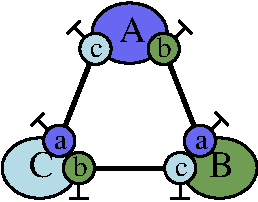
\includegraphics{generated_pictures/abc_contact_map.pdf}}\vspace*{2.5mm}\smallskip\\%
\end{minipage}
  }
  \subfigure[Triangle \agentfont{ABC}.]{%
  \begin{minipage}{0.25\linewidth}
    \label{fig:abc:triangle}
  \centering\scalebox{0.6}{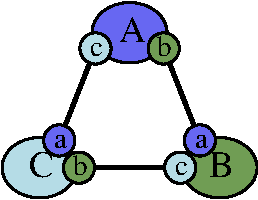
\includegraphics{generated_pictures/abc_triangle.pdf}}\vspace*{2.5mm}\smallskip\\%
\end{minipage}
  }
  \subfigure[A repeatable pattern.]{%
  \begin{minipage}{0.45\linewidth}
    \label{fig:abc:pattern}
    \vspace*{0.6cm}
  \centering\scalebox{0.6}{
\includegraphics{generated_pictures/abc_pattern.pdf}}\vspace*{0.5cm}\smallskip\\%
\end{minipage}}
\caption{The \agentfont{ABC} example.
The contact map  (Fig.\ref{fig:abc:cm}) specifies a typing discipline.
It displays every kind of proteins and specifies their interfaces.
The contact map also provides the potential states of each site:
either free $\freesymbol$, or bound to another site (which is encoded as a link in the contact map).
In Fig.R\ref{fig:abc:triangle} describes a biomolecular compound that is compatible with the contact map. Every instance of proteins belong to the contact map. Their interfaces is the same as in the contact map.
Also any bond between two sites complies with the link that are explicitely written in the contact map.
In \ref{fig:abc:pattern} describes a repeatable pattern.
This pattern is compatible with the contact map and can be repeated in order to form arbitrarily large biomolecular species.
}
\end{figure}
\section{Case studies}
\label{sec:case-study}

In this section, we introduce some examples to explain intuitively why there may be an unbounded number of biomolecular compounds in a rule-based model.  We also explain why naive approaches cannot be use to prove that the number of biomolecular compounds is finite in a given model,  while identifying the pitfalls that shall be avoided to achieve this goal.

\subsection{Elementary cycles}

Let us start with a simple example. We consider a model involving three kinds of protein $A$, $B$, $C$. Each protein has two binding sites: the protein $A$ has the binding sites $b$ and $c$, the protein $B$ has the binding sites $a$ and $c$, and the protein $C$ has the binding sites $a$ and $b$. Each binding site may be free, or bound to another site. Only three kinds of bonds are possible: the site $b$ of an instance of the protein $A$ may be bound to the site $a$ of an instance of the protein $B$; the site $c$ of an instance of the  protein $B$ may be bound to the site $b$ of an instance of the protein $C$; and the site $a$ of an instance of the protein $C$ may be bound to the site $c$ of a protein $A$.

These assumptions are summarised in a graph in Fig.~\ref{fig:abc:cm}. This graph is called the contact map of the model. It describes every kind of protein and every sites in their interfaces. The potential state of each site is also indicated. In our model, every sites may be free: they are all tagged with the symbol $\freesymbol$. Potential bonds are indicated by the means of edges between pair of sites.  The contact map provides a type discipline.
Every biomolecular compound in our models shall satisfy the contraints the contact map encodes about the interface of agents, the potential states of sites, and their potential bindings. An example of biomolecular compound that is compatible with the contact map is drawed in Fig.~\ref{fig:abc:triangle}. This biomolecular compound is made of three proteins \agent{A}{}, \agent{B}{}, and \agent{C}{}{} that are bound pair-wise so as to form a triangular shape.
In a biomolecular compound, every site shall be either free, or bound to at most one other site (but not both). In general, a biomolecular compound may not contain each kind of proteins. Also it may contain several instances of a given one.

The contact map that is given in Fig.~\ref{fig:abc:cm} is compatible with an infinite number of different (i.e.~\emph{non isomorphic}) molecular compounds.
Indeed we show in Fig.~\ref{fig:abc:pattern}, a pattern
that may be repeated an unbounded number of times in order to form arbitrary many different biomolecular compounds. This is tempting to relate the potential presence of an arbitrary number of different biomolecular compounds to the presence of a cycle in the contact map. However we shall see in the next examples that this intuition is misleading.


\begin{figure}
  \subfigure[Contact map.]{%
  \begin{minipage}{0.3\linewidth}
      \label{fig:self:cm}
  \centering\scalebox{0.6}{
\includegraphics{generated_pictures/self_contact_map.pdf}}\vspace*{2.5mm}\smallskip\\%
\end{minipage}
  }
  \subfigure[Exhaustive list of molecular compounds.]{%
  \begin{minipage}{0.6\linewidth}
    \label{fig:self:species}
  \centering\hfill\scalebox{0.6}{
\includegraphics{generated_pictures/self_monomer.pdf}}\hfill\scalebox{0.6}{
\includegraphics{generated_pictures/self_dimer.pdf}}\hfill\mbox{}\vspace*{2.5mm}\smallskip\\%
\end{minipage}}
\caption{The example of a protein that may form monomers and dimers.
The contact map (Fig.\ref{fig:self:cm}) contains a cycle, since the unique site of an instance of a  protein may be linked to the unique site of another instance of another protein. However, only once instance of this cycle may occur in a given biomolecular compound and the number of biomolecular compound remains bounded despite this cycle (Fig.~\ref{fig:self:species}).}
\end{figure}

\begin{figure}
  \subfigure[Contact map.]{%
  \begin{minipage}{0.45\linewidth}
      \label{fig:twoself:cm}
  \centering\scalebox{0.6}{
\includegraphics{generated_pictures/twoself_contact_map.pdf}}\vspace*{2.5mm}\smallskip\\%
\end{minipage}
  }
  \subfigure[A repeatable pattern.]{%
  \begin{minipage}{0.45\linewidth}
    \label{fig:twoself:pattern}
  \centering\scalebox{0.6}{
\includegraphics{generated_pictures/twoself_pattern.pdf}}\vspace*{2.5mm}\smallskip\\%
\end{minipage}}
\caption{An example of a protein with two sites \sitefont{a} and \sitefont{b} such that the site \sitefont{a} of a protein may be bound to the site \sitefont{a} of another protein and the site \sitefont{b} may be bound to the site \sitefont{b} of another protein.
The contact map (Fig.\ref{fig:twoself:cm}) contains two self-loops.
The pattern that is made of three proteins, the first two bound via their respective site \sitefont{a} and the last two bound via their respective site
\sitefont{b} is a repeatable patterns. Thus, an infinite number of biomolecular compounds is compatible with the contact map. Hence, in general, it is unsafe to discard self-loops from the contact map. }
\end{figure}

\subsection{Self loops}

In a second example we consider a model with only one kind of protein. This protein has a single site which may be either free, or bound to the site of another protein of the same kind. Roughly speaking a protein may form a monomer (when its site is free), or belongs to a dimer (when its site is bound). These assumptions are encoded in the contact map that is given in Fig.~\ref{fig:self:cm}. We notice that this contact map contains a cycle (from the unique site of the protein to itself). Indeed only the two biomolecular compounds that are depicted in Fig.~\ref{fig:self:species} are compatible with this contact map. Thus there is a finite number of them despite the cycle of the contact map.

One could think that self-loops should not be considered as cycles when trying to prove that the number of biomolecular compounds of a model is finite. Indeed whenever a molecular compound countains a bond that coresponds to a self-loop in the contact map, then both sites are necessarily  bound together and they are no longer available to form links with other sites. Yet the contact map that is given in Fig.~\ref{fig:twoself:cm} shows that it is unsafe in general  to discard the self-loops of the contact map. In this example, we consider only one kind of protein with two sites. Each site may be either free, or bound to the same site of another instance of the protein. It is then possible to form a chain a three proteins (see Fig.~\ref{fig:twoself:pattern}) that may be repeated an arbitrary number of times in a biomolecular compounds.

\subsection{Conflicting bindings}

It may happen that a site may be bound to several kinds of sites.
In the contact map, this site may connected to several edges which may be a part of cycle. However, every instance of such a site may be bound to at most
one site in a biomolecular compound. Thus some of such cycles may be not realisable in a biomolecular compound.



\subsection{Early events in the epidermic growth factor pathway}

\begin{figure}[t]
\subfigure[Contact map.]{%
\label{fig:cm}
\begin{minipage}{0.5\linewidth}%
\begin{center}
  \scalebox{0.4}{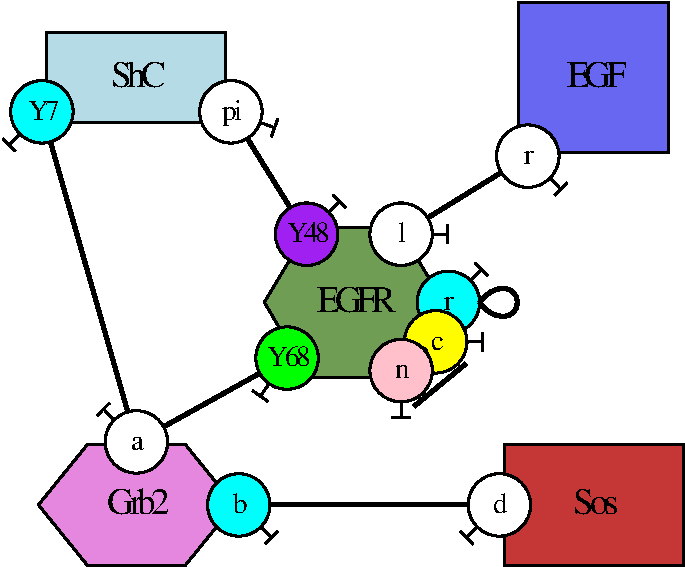
\includegraphics{generated_pictures/contact_map.pdf}}\vspace*{2.5mm}\smallskip\\%
\end{center}
\end{minipage}%
}
\subfigure[A biomolecular compound.]{%
\label{fig:sigma}
\begin{minipage}{0.5\linewidth}%
\begin{center}\scalebox{0.4}{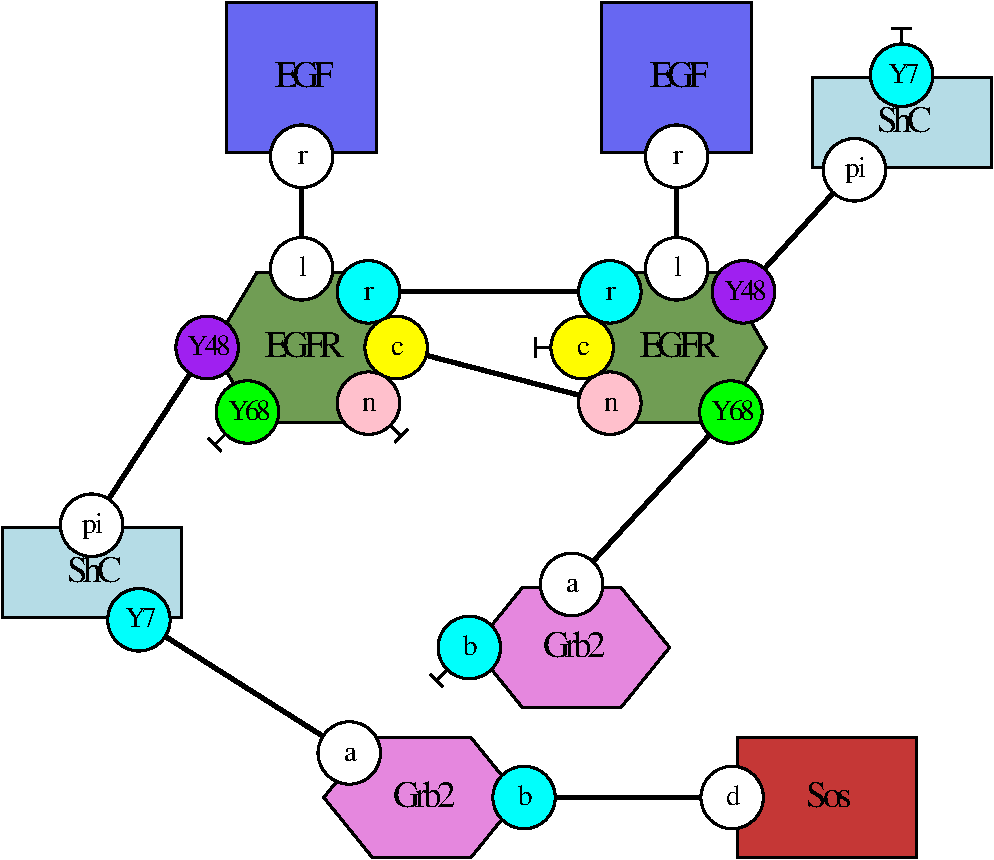
\includegraphics{generated_pictures/species.pdf}}\smallskip\\\end{center}%
\end{minipage}}
\caption{The example }
 \end{figure}

So far, we have considered only minimal case studies to try to understand which conditions are necessary on a contact map to be compatible with an infinite number of biomolecular species. In Fig.~\ref{cm:egfr},


\subsection{Clique}













\section{Site-graphs}

\label{sec:kappa}

In this section, we give some reminders about Kappa.
Since we focus on counting some specific occurrences of patterns, we do not introduce the full semantics of Kappa. Instead, we introduce only the notions of site-graphs and of embeddings among them, and we omit the notions of rule and of rule applications. We also omit internal states, since dealing with them would raise no difficulty.  We refer to
\cite{DBLP:journals/tcs/DanosL04,Feret_IJSI2013} for a more complete description of Kappa.

\subsection{Signature}

Firstly we define the signature of a model.
\begin{defn}[signature]
\label{def:signature}
A signature is a triple $\signaturesymb\bydef\signaturetuple$ where: \begin{enumerate}\item $\agentname$ is a finite set of agent types, \item $\sitename$ is a finite set of site identifiers; \item $\linksite\;:\;\agentname \rightarrow \wp(\sitename)$ is a site map.
\end{enumerate}\end{defn}


Agent types in $\agentname$ denote agents of interest, as kinds of proteins for instance.
Site identifiers in $\sitename$ represent identified loci for capabilities of interactions.
Agent types $A\in\agentname$ are associated with sets of sites $\linksite(A)$ which may be linked.

\begin{myexample}[signature]
\label{ex:signature}We define the signature for the model of the early events in the epidermic growth factor:
\begin{equation*}\signaturesymb\bydef\signaturetuple\end{equation*} where:
 \begin{enumerate}
 \item $\agentname \bydef \{\text{\agent{EGF}{}},\text{\agent{EGFR}{}},\text{\agent{Grb2}{}},\text{\agent{ShC}{}},\text{\agent{Sos}{}}\}$;
 \item $\sitename \bydef \{\text{\site{a}{}{}},\text{\site{b}{}{}},\text{\site{c}{}{}},
 \text{\site{d}{}{}},
\text{\site{n}{}{}},
 \text{\site{l}{}{}},
 \text{\site{pi}{}{}},
 \text{\site{r}{}{}},
 \text{\site{Y7}{}{}},\text{\site{Y48}{}{}},\text{\site{Y68}{}{}}\}$;
 \item $\linksite \bydef \map{%
 \begin{cases}
   \begin{array}{ccc}\agentname &\rightarrow & \wp(\sitename) \cr
   \text{\agent{EGF}{}}&\mapsto& \{\text{\site{r}{}{}}\}\cr
   \text{\agent{EGFR}{}}&\mapsto& \{\text{\site{c}{}{}},
  \text{\site{n}{}{}},
   \text{\site{l}{}{}},
   \text{\site{r}{}{}},
  \text{\site{Y48}{}{}},\text{\site{Y68}{}{}}\}\cr
\text{\agent{Grb2}{}}&\mapsto & \{\text{\site{a}{}{}},\text{\site{b}{}{}}\}\cr
\text{\agent{ShC}{}}&\mapsto &
\{\text{\site{pi}{}{},\site{Y7}{}{}}\}\cr
\text{\agent{Sos}{}}&\mapsto &
\{\text{\site{d}{}{}}\} \cr\end{array}\end{cases}}{[\text{\agent{EGF}{}}\mapsto \{\text{\site{r}{}{}}\},
\text{\agent{EGFR}{}}\mapsto \{\text{\site{c}{}{}},
\text{\site{n}{}{}},
\text{\site{l}{}{}},
\text{\site{r}{}{}},
\text{\site{Y48}{}{}},\text{\site{Y68}{}{}}\},
\text{\agent{Grb2}{}}\mapsto \{\text{\site{a}{}{}},\text{\site{b}{}{}}\},
\text{\agent{ShC}{}}\mapsto
\{\text{\site{pi}{}{},\site{Y7}{}{}}\},
\text{\agent{Sos}{}}\mapsto
\{\text{\site{d}{}{}}\}]}$
 \end{enumerate}
%  The agent types \agent{A}{}, \agent{B}{}, and \agent{C}{} denote the three kinds of proteins. Each instance of the protein \agent{A}{} has three sites the identifiers of which range from $1$ to $3$;
%  each instance of the protein \agent{B}{} has four sites the identifiers  of which range from $1$ to $4$; and each instance of the protein \agent{C}{} has two sites the identifiers of which range from $1$ to $2$.
\end{myexample}

\subsection{$\Sigma$-graphs and morphisms among $\Sigma$-graphs}


$\Sigma$-graphs are graphs the nodes of which are typed agents with some sites which may bear sets of binding states. In general, $\Sigma$-graphs encode some  specific type disciplines \cite{DBLP:journals/mscs/DanosHW13}: they summarise the potential bonds and provide contextual conditions over them \cite{Camporesi:CMSB2013}. Patterns and bio-molecular compounds are specific kinds of $\Sigma$-graphs.


\begin{figure}[t]
\subfigure[A morphism from $\graphsymb_{\Sigma}$ into $\graphsymb_{\textit{CM}}$.]{%
\label{fig:morphism}
\begin{minipage}{\linewidth}%
\vspace*{0.6cm}
\begin{center}\scalebox{0.4}{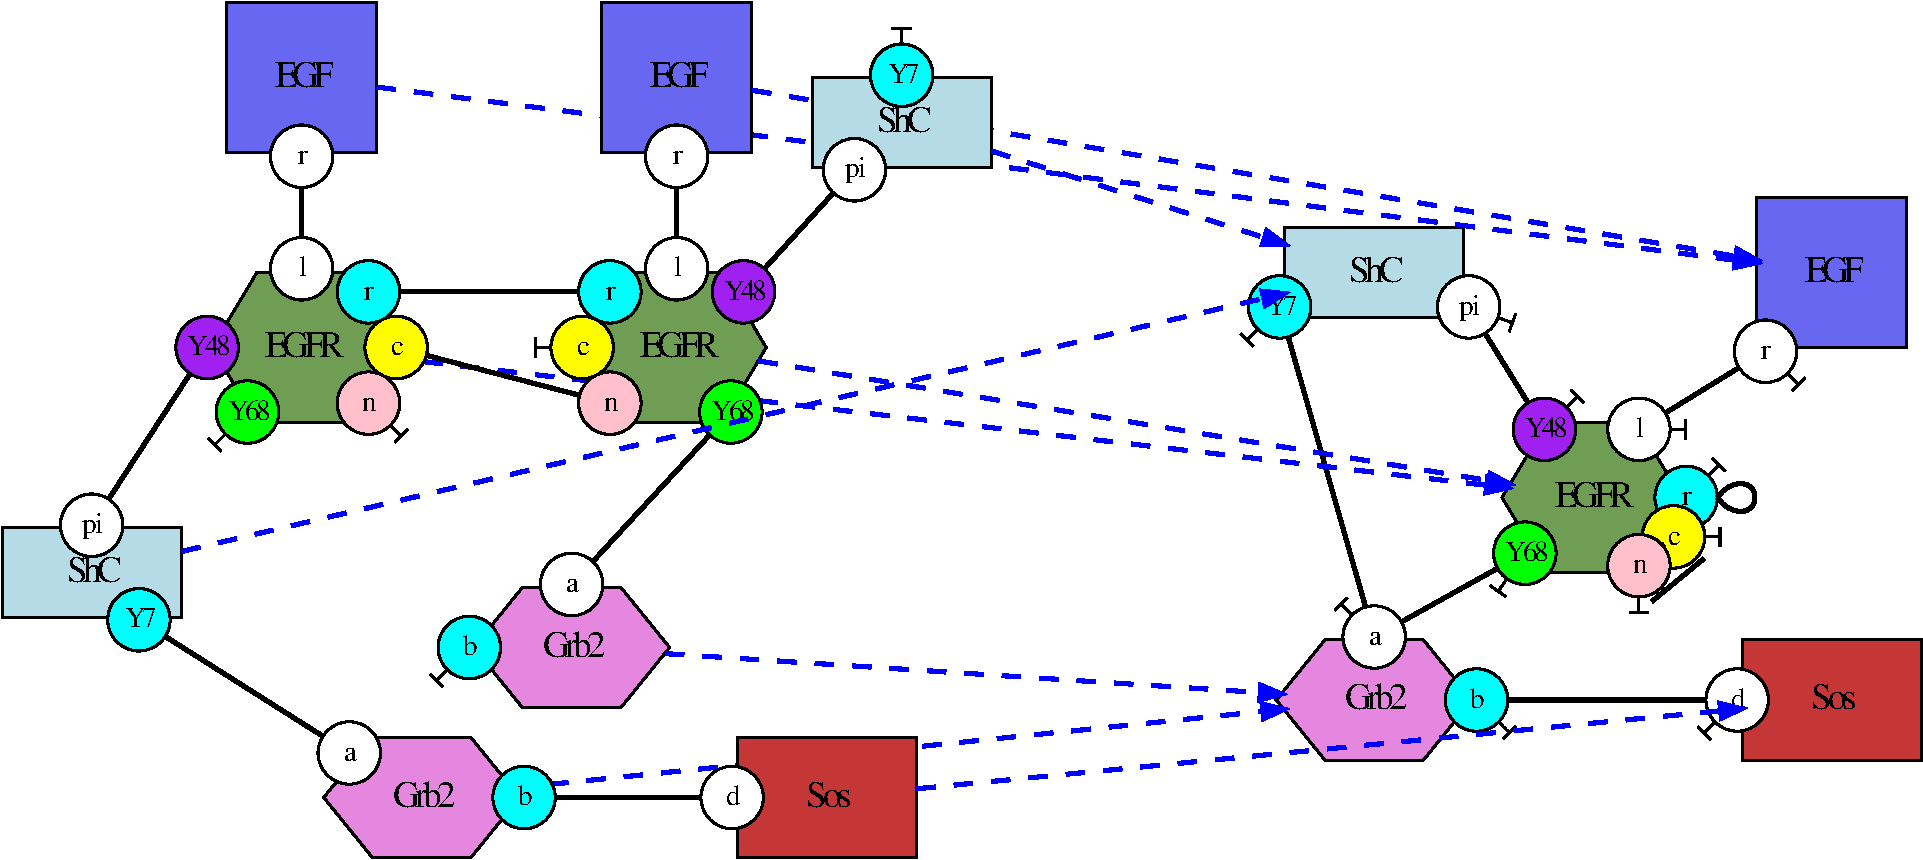
\includegraphics{generated_pictures/species_cm.pdf}}\smallskip\\%\vspace*{0.55cm}
\end{center}%
\end{minipage}}

\caption{Two $\Sigma$-graphs $\graphsymb_{\textit{CM}}$ and
$\graphsymb_{\textit{SP}}$, and a morphism from $\graphsymb_{\textit{CM}}$ to $\graphsymb_{\Sigma}$. The $\Sigma$-graph $\graphsymb_{\textit{CM}}$ is a contact map. It provides context-insensitive information about the potential state of each binding site. The $\Sigma$-graph $\graphsymb_{\textit{SP}}$ is a biomolecular species. It containts several instances of some proteins.
Every sites is documented in each protein instance and each site is either free, or bound to another site. The morphism between $\graphsymb_{\textit{CM}}$ and $\graphsymb_{\textit{SP}}$ smashes all
the proteins of the $\Sigma$-graph $\graphsymb_{\textit{SP}}$ according to their type. This is the unique morphism from the site graph $\graphsymb_{\textit{CM}}$ into the site-graph $\graphsymb_{\textit{SP}}$.
}
\label{fig:sigma-graphs}
\end{figure}

\begin{defn}[$\Sigma$-graphs]\label{def:summary}
A $\Sigma$-graph is a tuple $\graphsymb\bydef\graphtuple[G]$ where:
\begin{enumerate}
\item $\agents[G]\subseteq \mathbb{N}$ is a finite set of agents,
\item $\type[G]\;:\;\agents\rightarrow \agentname$ is a function mapping each agent to its type,
\item $\sites[G]$ is a subset of the set $\{(n,i)\;|\; n\in \agents, i\in\linksite(\type[G](n))\}$,
\item $\links[G]$ is a function between the set $\sites$ and the set
 $\wp(\sites\cup\ext)$  such that for any two sites $(n,i),(n',i')\in\sites$, we have $(n',i')\in\links[G](n,i)$ if and only if $(n,i)\in\links[G](n',i')$.
\end{enumerate}
\end{defn}

The set $\sites$ denotes the set of binding sites.
Whenever $\freesymbol\;\in\links(n,i)$, the site $(n,i)$ may be free.
Various levels of information may be given about the sites that are bound.
Whenever $\bound{}\in\links(n,i)$, the site $(n,i)$ may be bound to an unspecified site.
Whenever $(n',i')\in\links(n,i)$ (and hence $(n,i)\in\links(n',i')$), the sites $(n,i)$ and $(n',i')$ may be bound together.

For a $\Sigma$-graph $\graphsymb$, we write as $\agents[\graphsymb]$ its set of agents, $\type[\graphsymb]$ its typing function, $\sites[\graphsymb]$ its set of sites, and $\links[\graphsymb]$ its set of links.

\begin{myexample}[$\Sigma$-graph]
We give two examples of $\Sigma$-graph. We consider the $\Sigma$-graph $\graphsymb_\textit{CM}%\bydef\graphtuple[\graphsymb_\textit{CM}]
$ that is defined as follows:
\begin{enumerate}
  \item $\agents[\graphsymb_\textit{CM}]\bydef\{1,2,3,4,5\}$;
  \item $\type[\graphsymb_\textit{CM}]\bydef \map{\begin{cases}\begin{array}{ccc}%
  1 &\mapsto&\agent{EGF}{}\cr%
  2 &\mapsto&\agent{EGFR}{}\cr%
  3 &\mapsto&\agent{Grb2}{}\cr%
  4 &\mapsto&\agent{ShC}{}\cr%
  5 &\mapsto&\agent{Sos}{}\cr%
\end{array}\end{cases}}{[1 \mapsto \agent{EGF}{}, 2  \mapsto \agent{EGFR}{}, 3 \mapsto \agent{Grb2}{}, 4 \mapsto \agent{ShC}, 5 \mapsto \agent{Sos}];}$
  \item $\sites[\graphsymb_\textit{CM}]\bydef
\bigcup \{(n,i)\;|\; n\in \agents[\graphsymb_\textit{CM}],
i\in\linksite(\type[\graphsymb_{\textit{CM}}])\}$;
  \item $\links[\graphsymb_\textit{CM}]\bydef\map{}{\left[%
  \begin{array}{l}
    (\text{\agent{EGF}{}},\text{\site{r}{}{}})\mapsto \{\freesymbol,\},\cr
    (\text{\agent{EGFR}{}},\text{\site{l}{}{}})\mapsto \{\freesymbol,\},\cr
    (\text{\agent{EGFR}{}},\text{\site{r}{}{}})\mapsto \{\freesymbol,\},\cr
    (\text{\agent{EGFR}{}},\text{\site{c}{}{}})\mapsto \{\freesymbol,\},\cr
    (\text{\agent{EGFR}{}},\text{\site{n}{}{}})\mapsto \{\freesymbol,\},\cr
    (\text{\agent{EGFR}{}},\text{\site{Y48}{}{}})\mapsto \{\freesymbol,\},\cr
    (\text{\agent{EGFR}{}},\text{\site{Y68}{}{}})\mapsto \{\freesymbol,\},\cr
    (\text{\agent{Grb2}{}},\text{\site{a}{}{}})\mapsto \{\freesymbol,\},\cr
    (\text{\agent{Grb2}{}},\text{\site{b}{}{}})\mapsto \{\freesymbol,\},\cr
    (\text{\agent{ShC}{}},\text{\site{pi}{}{}})\mapsto \{\freesymbol,\},\cr
    (\text{\agent{ShC}{}},\text{\site{Y7}{}{}})\mapsto \{\freesymbol,\},\cr
    (\text{\agent{Sos}{}},\text{\site{d}{}{}})\mapsto \{\freesymbol,\},\cr
  \end{array}\right]}$.
\end{enumerate}
and the $\Sigma$-graph $\graphsymb_{\Sigma}%$\bydef\graphtuple[\graphsymb_{\Sigma}]
$ that is defined as follows:
\begin{enumerate}
  \item $\agents[\graphsymb_{\Sigma}]\bydef\{1,2,3,4\}$;
  \item $\type[\graphsymb_{\Sigma}]\bydef \map{\begin{cases}\begin{array}{ccc}%
  1 &\mapsto&\agent{A}{}\cr%
  2 &\mapsto&\agent{A}{}\cr%
  3 &\mapsto&\agent{B}{}\cr%
  4 &\mapsto&\agent{C}{}\cr%
\end{array}\end{cases}}{[1 \mapsto \agent{A}{}, 2 \mapsto \agent{A}{}, 3 \mapsto \agent{B}{}, 4 \mapsto \agent{C}{}\;];}$
  \item $\sites[\graphsymb_{\Sigma}]\bydef\left\{\begin{array}{l}(1,1),(1,2),(1,3),(2,1),(2,2),(2,3),\cr(3,1),(3,2),(3,3),(3,4),(4,1),(4,2)\end{array}\right\}$;
  \item $\links[\graphsymb_{\Sigma}]\bydef\map{}{\left[%
  \begin{array}{l}
    (1,1)\mapsto\{%\freesymbol,
    (3,1)\},
    (1,2)\mapsto\{\freesymbol,(3,2),(3,3)\},
    (1,3)\mapsto\{%\freesymbol,
    (3,3),(4,2)\},\cr%
    (2,1)\mapsto\{\freesymbol\},
    (2,2)\mapsto\{\freesymbol,(3,2),(3,3)\},
    (2,3)\mapsto\{\freesymbol,(3,3),(4,2)\},\cr%
    (3,1)\mapsto\{\freesymbol,(1,1)\},
    (3,2)\mapsto\{\freesymbol,(1,2),(2,2)\},\cr (3,3)\mapsto\{\freesymbol,(1,2),(1,3),(2,2),(2,3)\},
    (3,4)\mapsto\{\freesymbol,(4,1)\},\cr%
    (4,1)\mapsto\{\freesymbol,(3,4)\},
    (4,2)\mapsto\{\freesymbol,(1,3),(2,3)\}
  \end{array}\right]}.$
\end{enumerate}
The $\Sigma$-graphs $\graphsymb_{\textit{CM}}$ and $\graphsymb_{\Sigma}$
are graphically described respectively in Figs.~\ref{fig:cm} and \ref{fig:sigma}. We notice that agent identifiers are omitted (an agent is identified by its position). Site identifiers are omitted. Sites are depicted in increasing order of their identifiers from bottom up.

The $\Sigma$-graph $\graphsymb_{\textit{CM}}$ plays a specific role: we call it the contact map of the model. In a contact map each agent type occurs exactly once and each agent documents its full set of sites. It can be
interpreted as a context-insensitive description of the potential bindings
between sites of agents.
\end{myexample}


$\Sigma$-graphs may be related by structure-preserving maps of agents, called morphisms. The definition of a morphism between two $\Sigma$-graphs  is given as follows:
\begin{defn}[morphisms]
 A \emph{morphism} $h\;:\;G\;\rightarrow H$ from the $\Sigma$-graph $G$ into the $\Sigma$-graph $H$ is a function of agents $h\;:\;\agents[G]\rightarrow \agents[H]$ satisfying,
for all agent identifiers $n$, $n'\in\agents[G]$, for all site identifiers $i\in\linksite(\type[G](n))$, $i'\in\linksite(\type[G](n'))$:
\begin{enumerate}
\item $\type[G](n) = \type[H](h(n))$;
\item if $(n,i)\in\sites[G]$, then $(h(n), i)\in\sites[H]$;
\item if $(n',i')\in\links[G](n,i)$, then $(h(n'),i')\in\links[H](h(n),i)$;
\item if \;$\freesymbol{ }\in\links[G](n,i)$, then \;$\freesymbol{ }\in\links[H](h(n),i)$;
\item if $\bound{}\in\links[G](n,i)$, then  $\links[H](h(n),i)\cap\{\bound{}\}\cup\sites[H]\neq\emptyset$.
\end{enumerate}
\end{defn}

Morphisms preserve the type of agents.
They also preserve each agent set of sites, but more sites may be documented in the image of the morphism. A site that may be free shall be mapped to a site that may be free. Two sites that may be bound together shall be mapped to two sites that may be bound together. Lastly, whenever a site may be bound to an unspecified site, it shall be mapped to a site that is bound to either an unspecified or a specified (or both) one.

\begin{myexample}[morphisms]
The following function: $[1 \mapsto 1, 2 \mapsto 1, 3\mapsto 2, 4\mapsto 3]$ induces a morphism from the $\Sigma$-graph $\graphsymb_{\Sigma}$ into the $\Sigma$-graph $\graphsymb_{\textit{CM}}$. This morphism is graphically described in Fig.~\ref{fig:morphism}. We notice that both agents of type \agentfont{A} have been merged into a single agent in the contact map, while merging the potential states of their sites. This way, the contact map
provides a coarser
(context-insensitive) summary of potential bonds in a model.
\end{myexample}

Two morphisms from a $\Sigma$-graph  $E$ to a $\Sigma$-graph $F$, and from the $\Sigma$-graph $F$ to a $\Sigma$-graph $G$ respectively, compose in the usual way (and form a morphism from the $\Sigma$-graph $E$ into the
$\Sigma$-graph  $G$).

\subsection{Patterns and embeddings}

Now we restrict the definition of $\Sigma$-graphs so as to
focus on the ones that may express parts of the state of the system.
These $\Sigma$-graphs, that we call patterns, are defined as follows:

\begin{figure}[t]

\subfigure[The pattern $P$.]{%
\label{fig:pattern}
\begin{minipage}{\keep{\explainweakembedding}{0.3}{0.2}\linewidth}%
\vspace*{16mm}\begin{center}
%  \scalebox{0.4}{\includegraphics{generated_pictures/pattern.pdf}}\vspace*{3mm}\vspace*{0.45cm}\smallskip\\%
\end{center}
\end{minipage}}
\keep{\explainweakembedding}{\subfigure[The pattern $P'$.]{%
\label{fig:patternbis}
\begin{minipage}{0.3\linewidth}%
\vspace*{8mm}\begin{center}
%  \scalebox{0.4}{\includegraphics{generated_pictures/patternprime.pdf}}
  \vspace*{29.3mm}\smallskip\\%
\end{center}
\end{minipage}}}{}
\subfigure[The biomolecular compound $S$.]{%
\label{fig:species}
\begin{minipage}{0.3\linewidth}%
  \vspace*{8mm}
\begin{center}\scalebox{0.4}{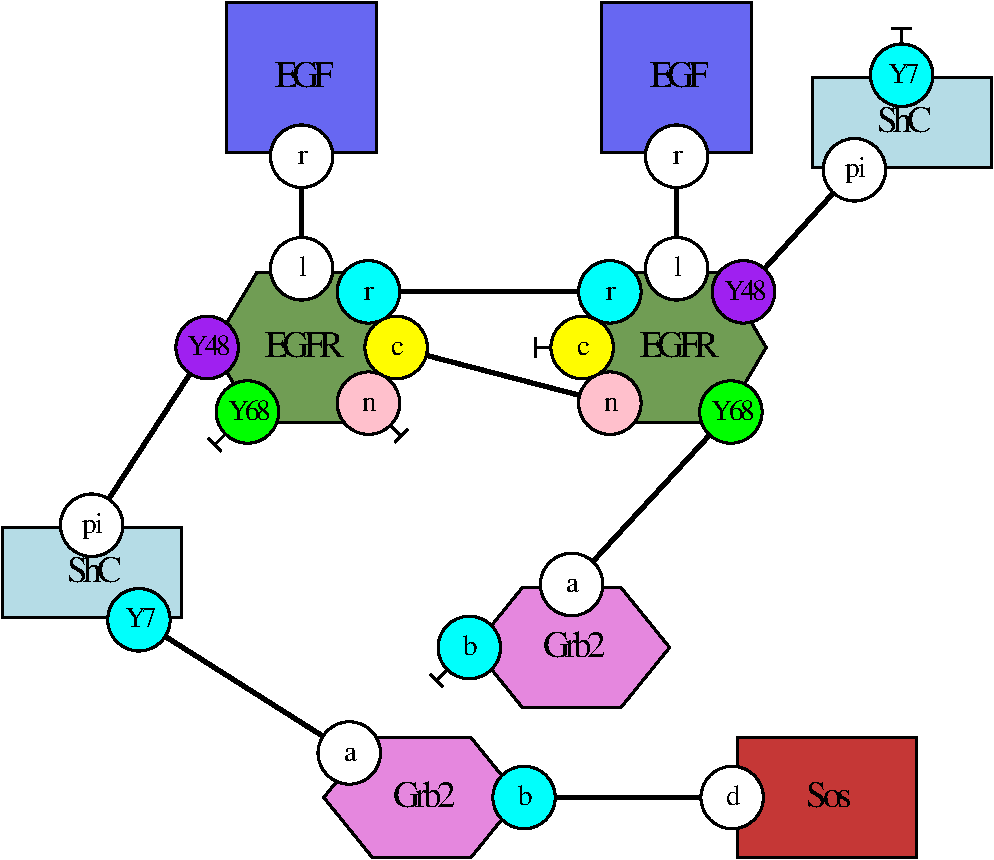
\includegraphics{generated_pictures/species.pdf}}\vspace*{3.8mm}\smallskip\\\end{center}%
\end{minipage}}%
\keep{\explainweakembedding}{

}{}%
\subfigure[An embedding from $P$ into $S$.]{%
\label{fig:embedding}
\begin{minipage}{0.45\linewidth}%
\begin{center}%\scalebox{\keep{\explainweakembedding}{0.6}{0.6}}{\includegraphics{generated_pictures/embedding.pdf}}\smallskip\\
  \end{center}%
\end{minipage}}
%\keep{\explainweakembedding}{\subfigure[A weak emnbedding from $P'$ into $S'$.]{%
%\label{fig:weakembedding}
%\begin{minipage}{0.45\linewidth}
%  \begin{center}
%      \scalebox{\keep{\explainweakembedding}{0.6}{0.6}}{\includegraphics{generated_pictures/weak_embedding.pdf}}\smallskip\\
%  \end{center}
%\end{minipage}}}{}
\caption{\keep{\explainweakembedding}{Three}{Two} patterns $P$\keep{\explainweakembedding}{, $P'$,}{} and $S$,  \keep{\explainweakembedding}{}{and} an embedding from the pattern $P$ to the biomolecular compound $S$\keep{\explainweakembedding}{, and a weak embedding from the pattern $P'$ to the biomolecular compound $S$}{}. \keep{\explainweakembedding}{There is no embedding from $P'$ to $S$.}{} The pattern $S$ is a species: it forms a connected component and the state of each site in  each agent is fully documented.}
\label{fig:patterns}
\end{figure}


\begin{defn}[patterns]
A pattern is a $\Sigma$-graph $P$ such that, for every site $s\in\sites[P]$ both following conditions are satisfied:
\begin{enumerate}
\item the set $\links[P](s)$ contains at most one element;
\item the set $\links[P](s)$ does not contain the element $s$.
\end{enumerate}
\end{defn}
The first condition ensures that the state of every site is either unspecified,
or free, or bound to an unspecified site, or bound to a single specific site. The second condition ensures that a site is never bound to itself.


\begin{myexample}[patterns]
We give \keep{\explainweakembedding}{three}{two} examples of patterns. We consider the pattern $P%\bydef\graphtuple[P]
$ that is defined as follows:
\begin{enumerate}
  \item $\agents[P]\bydef\{1\}$;
  \item $\type[P]\bydef [1 \mapsto \agent{A}{}]$;
  \item $\sites[P]\bydef\{(1,1),(1,3)\}$;
  \item $\links[P]\bydef [(1,1)\mapsto \{\bound{}\}, (1,3)\mapsto \{\freesymbol{}\}]$\keep{\explainweakembedding}{,}{;}
\end{enumerate}
\keep{\explainweakembedding}{the pattern $P'%\bydef\graphtuple[P']
$ that is defined as follows:
\begin{enumerate}
  \item $\agents[P']\bydef\{1\}$;
  \item $\type[P']\bydef [1 \mapsto \agent{A}{}]$;
  \item $\sites[P']\bydef\{(1,3)\}$;
  \item $\links[P']\bydef [(1,3)\mapsto \{\freesymbol\}]$;
\end{enumerate}}{}
and the pattern $S%\bydef\graphtuple[S]
$ that is defined as follows:
\begin{enumerate}
  \item $\agents[S]\bydef\{1,2,3,4\}$;
  \item $\type[S]\bydef [1 \mapsto \agent{A}{}, 2 \mapsto \agent{A}{}, 3 \mapsto \agent{B}{}, 4 \mapsto \agent{C}{}]$;
  \item $\sites[S]\bydef\left\{\begin{array}{l}(1,1),(1,2),(1,3),(2,1),(2,2),(2,3),\cr
  (3,1),
                               (3,2),(3,3),(3,4),(4,1),(4,2)\end{array}\right\}$;
  \item $\links[S]\bydef
\left[\begin{array}{l}
      (1,1)\mapsto\{(3,1)\},
      (1,2)\mapsto\{(3,2)\},
      (1,3)\mapsto\{\freesymbol\},\cr
      (2,1)\mapsto\{\freesymbol\},
      (2,2)\mapsto\{(3,3)\},
      (2,3)\mapsto\{\freesymbol\},\cr
      (3,1)\mapsto\{(1,1)\},
      (3,2)\mapsto\{(1,2)\},
      (3,3)\mapsto\{(2,2)\},
      (3,4)\mapsto\{(4,1)\},\cr
      (4,1)\mapsto\{(3,4)\},
      (4,2)\mapsto\{\freesymbol{}\}\end{array}\right]$.
\end{enumerate}
The patterns $P$\keep{\explainweakembedding}{, $P'$,}{} and $S$
are graphically described respectively in Figs.~\ref{fig:pattern}\keep{\explainweakembedding}{,~\ref{fig:patternbis}}{}  and \ref{fig:species}.
\end{myexample}


A biomolecular compound is a connected pattern in which the state of each site is documented (no further information may be added). Depending on the choice of the semantics, the state of the system may be described either as a function from biomolecular compound to concentrations (differential setting), or as a multi-set of biomolecular compound  (stochastic setting).

Patterns may be related by embeddings. Besides preserving the structure of patterns, embeddings map agents to agents injectively.

\begin{defn}[embeddings]
  An embedding is a morphism from a pattern into another one, that is induced by an injective agent function.

  We denote as $[P,P']$ the set of the embeddings from a pattern $P$ to a pattern $P'$.
\end{defn}

\begin{myexample}[embeddings]
  The function $[1\mapsto 1]$ induces an embedding from the pattern $P$ to the biomolecular compound $S$, as depicted in Fig.~\ref{fig:embedding}. %There is no embedding from the pattern $P'$ to the pattern $S$.
\end{myexample}

As opposed to classical notions of embeddings between graphs, embeddings between patterns preserve the freeness of sites.

The composition of two embeddings is an embedding.

\section{Graph of sites}

\section{Graph of potential links}

\section{Taking into account the result of a static analysis}

\section{Conclusion}

\bibliographystyle{entcs}
\bibliography{polymers}

\end{document}
